\documentclass[iop]{emulateapj}
%%GB: General commands to make editing easier and with less typos.

%% -----------------------------------------------
%% Definition of a forloop command
%%
%% This is called via: 
%%   \forloop[step]{counter}{initial_value}{conditional}{code_block} 
%%
\newcommand{\forloop}[5][1]%
{%
\setcounter{#2}{#3}%
\ifthenelse{#4}%
	{%
	#5%
	\addtocounter{#2}{#1}%
	\forloop[#1]{#2}{\value{#2}}{#4}{#5}%
	}%
% Else 
	{%
	}%
}% 

%% -----------------------------------------------
%% Editing
\newcommand{\tbd}[1]{{\par\bf\textsc{TBD: #1\\}}}
\newcommand{\ctbd}[1]{}
\newcommand{\corr}{\textcolor{red}{(corr?) }}
\newcommand{\spl}{\textcolor{red}{(spl?) }}

%% ------------------------------------------------
%% Hun characters
\newcommand{\ii}{\'\i }
\newcommand{\oo}{\H{o}}
\newcommand{\uu}{\H u}

%% --------------------------------------
%% Often used. 
\newcommand{\lc}{light curve}
\newcommand{\lcs}{light curves}
\newcommand{\Lc}{Light curve}
\newcommand{\Lcs}{Light curves}
\newcommand{\avg}[1]{\ensuremath{\langle #1\rangle}}
\newcommand{\med}[1]{\ensuremath{\langle #1\rangle_{med}}}
\newcommand{\dpt}{data-point}
\newcommand{\dpts}{data-points}
\newcommand{\tel}{telescope}
\newcommand{\magn}{magnitude}
\newcommand{\stan}{standard}
\newcommand{\aper}{aperture}
\newcommand{\oot}{out-of-transit}
\newcommand{\OOT}{Out-of-Transit}
\newcommand{\cfa}{Harvard-Smithsonian Center for Astrophysics (CfA)}
\newcommand{\cfadigi}{CfA Speedometers}
\newcommand{\cmd}{color-magnitude diagram}

%% ---------------------------------------------
%% 
\newcommand{\conc}[1]{\noindent\par{\noindent{$\mathbf \Longrightarrow$ \bf #1}}}
\newcommand{\diam}{\ensuremath{\oslash}}
\newcommand{\ccdsize}[1]{\ensuremath{\rm #1\times\rm#1}}
\newcommand{\fovsize}[2]{\ensuremath{\rm #1 #2\times\rm#1 #2}}
\newcommand{\tsize}[1]{\mbox{\rm #1 m}}
\newcommand{\band}[1]{\ensuremath{#1}~band}
\newcommand{\sband}[1]{\ensuremath{#1}}
\newcommand{\ordo}{\ensuremath{\mathcal{O}}}
\newcommand{\chisq}{\ensuremath{\chi^2}}
\newcommand{\RA}[3]{\ensuremath{#1^{\mathrm h}#2^{\mathrm m}#3^{\mathrm s}}}
\newcommand{\DEC}[3]{\ensuremath{#1^{\mathrm d}#2^{\mathrm m}#3^{\mathrm s}}}

%% ---------------------------------------------------------------------
%% Dimensions/quantities
\newcommand{\ghr}{\ensuremath{^h}}
\newcommand{\gmin}{\ensuremath{^m}}
\newcommand{\Ks}{\ensuremath{K_s}}
\newcommand{\masy}{\ensuremath{\rm mas\,yr^{-1}}}
\newcommand{\kms}{\ensuremath{\rm km\,s^{-1}}}
\newcommand{\ms}{\ensuremath{\rm m\,s^{-1}}}
\newcommand{\msd}{\ensuremath{\rm m\,s^{-1}\,d^{-1}}}
\newcommand{\mss}{\ensuremath{\rm m\,s^{-2}}}
\newcommand{\gcmc}{\ensuremath{\rm g\,cm^{-3}}}
\newcommand{\ergscmsq}{\ensuremath{\rm erg\,s^{-1}\,cm^{-2}}}
\newcommand{\C}{\ensuremath{^{\circ}C\;}}
\newcommand{\el}{\ensuremath{e^-}}
\newcommand{\sqarcsec}{\ensuremath{\Box^{\prime\prime}}}
\newcommand{\sqarcdeg}{\ensuremath{\Box^{\circ}}}
\newcommand{\pxs}{\ensuremath{\rm \arcsec pixel^{-1}}}
\newcommand{\aduel}{\ensuremath{\lbrack ADU/\el \rbrack}}
\newcommand{\eladu}{\ensuremath{\lbrack \el/ADU \rbrack}}
\newcommand{\adupixs}{\ensuremath{\rm ADU/(pix\, s)}}
\newcommand{\elpixs}{\ensuremath{\rm \el/(pix\, s)}}
\newcommand{\masyr}{\ensuremath{\rm mas\,yr^{-1}}}
%\newcommand{\arcdeg}{\ensuremath{^{\circ}}}


%% ---------------------------------------------------------------------
%% General
\newcommand{\msini}{\ensuremath{m \sin i}}
\newcommand{\mplsini}{\ensuremath{\mpl\sin i}}
\newcommand{\teff}{\ensuremath{T_{\rm eff}}}
\newcommand{\logg}{\ensuremath{\log{g}}}
\newcommand{\vsini}{\ensuremath{v \sin{i}}}
\newcommand{\feh}{\ensuremath{\rm [Fe/H]}}
\newcommand{\logl}{\ensuremath{\log{L}}}
\newcommand{\vmac}{\ensuremath{v_{\rm mac}}}
\newcommand{\vmic}{\ensuremath{v_{\rm mic}}}
% Activity index R'_HK
\newcommand{\rhk}{\ensuremath{R^{\prime}_{\rm HK}}}
% log of R'_HK
\newcommand{\logrhk}{\ensuremath{\log\rhk}}
% S average value
\newcommand{\Savg}{\ensuremath{\langle S\rangle}}
% Some magnitude differences
\newcommand{\vic}{\ensuremath{V\!-\!I_C}}
\newcommand{\ebv}{\ensuremath{E(B\!-\!V)}}

%% ---------------------------------------------------------------------
%% Solar quantities 
\newcommand{\rsun}{\ensuremath{R_\odot}}
\newcommand{\msun}{\ensuremath{M_\sun}}
\newcommand{\lsun}{\ensuremath{L_\sun}}
\newcommand{\loglsun}{\ensuremath{\log{L_\sun}}}
\newcommand{\teffsun}{\ensuremath{T_{eff,\sun}}}
\newcommand{\rhosun}{\ensuremath{\rho_\sun}}
\newcommand{\loggsun}{\ensuremath{\log{g_{\sun}}}}

%% ---------------------------------------------------------------------
%% Stellar quantities 
\newcommand{\rstar}{\ensuremath{R_\star}}
\newcommand{\mstar}{\ensuremath{M_\star}}
\newcommand{\lstar}{\ensuremath{L_\star}}
\newcommand{\astar}{\ensuremath{a_\star}}
\newcommand{\loglstar}{\ensuremath{\log{L_\star}}}
\newcommand{\teffstar}{\ensuremath{T_{\rm eff\star}}}
\newcommand{\rhostar}{\ensuremath{\rho_\star}}
\newcommand{\loggstar}{\ensuremath{\log{g_{\star}}}}

%% ---------------------------------------------------------------------
%% Earth
\newcommand{\rearth}{\ensuremath{R_\oplus}}
\newcommand{\mearth}{\ensuremath{M_\oplus}}
\newcommand{\learth}{\ensuremath{L_\earth}}
\newcommand{\teffearth}{\ensuremath{T_{\rm eff,\earth}}}
\newcommand{\rhoearth}{\ensuremath{\rho_\earth}}

%% ---------------------------------------------------------------------
%% Planetary
\newcommand{\rpl}{\ensuremath{R_{p}}}
\newcommand{\mpl}{\ensuremath{M_{p}}}
\newcommand{\lpl}{\ensuremath{L_{p}}}
\newcommand{\teffpl}{\ensuremath{T_{\rm eff,{p}}}}
\newcommand{\rhopl}{\ensuremath{\rho_{p}}}
\newcommand{\ipl}{\ensuremath{i_{p}}}
\newcommand{\epl}{\ensuremath{e_{p}}}
\newcommand{\gpl}{\ensuremath{g_{p}}}
\newcommand{\loggpl}{\ensuremath{\log g_{p}}}

\newcommand{\arstar}{\ensuremath{a/\rstar}}
\newcommand{\zrstar}{\ensuremath{\zeta/\rstar}}

%% ---------------------------------------------------------------------
%% Jupiter
\newcommand{\rjup}{\ensuremath{R_{\rm J}}}
\newcommand{\mjup}{\ensuremath{M_{\rm J}}}
\newcommand{\ljup}{\ensuremath{L_{\rm J}}}
\newcommand{\teffjup}{\ensuremath{T_{eff,{\rm J}}}}
\newcommand{\rhojup}{\ensuremath{\rho_{\rm J}}}
\newcommand{\gjup}{\ensuremath{\g_{\rm J}}}

\newcommand{\rjuplong}{\ensuremath{R_{\rm Jup}}}
\newcommand{\mjuplong}{\ensuremath{M_{\rm Jup}}}
\newcommand{\ljuplong}{\ensuremath{L_{\rm Jup}}}
\newcommand{\teffjuplong}{\ensuremath{T_{eff,{\rm Jup}}}}
\newcommand{\rhojuplong}{\ensuremath{\rho_{\rm Jup}}}
\newcommand{\gjuplong}{\ensuremath{\g_{\rm Jup}}}

%% -----------------------------
%% Software
\newcommand{\pack}[1]{\textsc{\lowercase{#1}}}
\newcommand{\prog}[1]{\texttt{\lowercase{#1}}}
\newcommand{\iraf}{\pack{iraf}}
\newcommand{\todcor}{\prog{todcor}}
\newcommand{\xcsao}{\prog{xcsao}}
\newcommand{\daophot}{\pack{daophot}}
\newcommand{\fihat}{\pack{fihat}}
\newcommand{\fistar}{\prog{fistar}}
\newcommand{\fiphot}{\prog{fiphot}}
\newcommand{\grmatch}{\prog{grmatch}}
\newcommand{\grtrans}{\prog{grtrans}}

%% ---------------------------------------
%% References
%\newcommand{\pref}[1]{p.~\pageref{#1}}
%\newcommand{\figr}[1]{Fig.~\ref{fig:#1}}
%\newcommand{\secr}[1]{\mbox{\S\ \ref{sec:#1}}}
%\newcommand{\eqr}[1]{Eq.~\ref{eq:#1}}
%\newcommand{\tabsr}[1]{Tab.~\ref{tab:#1}}
%\newcommand{\tabr}[1]{\mbox{Table~\ref{tab:#1}}}
%\newcommand{\figrp}[1]{Fig.~\ref{fig:#1} on \pref{fig:#1}}
%\newcommand{\secrp}[1]{\S\ref{sec:#1} on \pref{sec:#1}}
%\newcommand{\eqrp}[1]{Eq.~\ref{eq:#1} on \pref{eq:#1}}
%\newcommand{\tabrp}[1]{Tab.~\ref{tab:#1} on \pref{tab:#1}}

\newcommand{\refp}[1]{p.~\pageref{#1}}

\newcommand{\reffig}[1]{Fig.~\ref{fig:#1}}
\newcommand{\refsec}[1]{\mbox{\S\ \ref{sec:#1}}}
\newcommand{\refeq}[1]{Eq.~\ref{eq:#1}}
\newcommand{\reftab}[1]{Tab.~\ref{tab:#1}}

\newcommand{\reffigl}[1]{Figure~\ref{fig:#1}}
\newcommand{\refsecl}[1]{\mbox{Section \ref{sec:#1}}}
\newcommand{\refeql}[1]{Equation~\ref{eq:#1}}
\newcommand{\reftabl}[1]{Table~\ref{tab:#1}}

\newcommand{\reffigp}[1]{\reffig{#1} on \pref{fig:#1}}
\newcommand{\refsecp}[1]{\refsec{#1} on \pref{sec:#1}}
\newcommand{\refeqp}[1]{\refeq{#1} on \pref{eq:#1}}
\newcommand{\reftabp}[1]{\reftab{#1} on \pref{tab:#1}}

\newcommand{\reffigls}[2]{Figures~\ref{fig:#1}--\ref{fig:#2}}
\newcommand{\reftabls}[2]{Tables~\ref{tab:#1}--\ref{tab:#2}}

%% --------------------------------------
%% Instruments
% 
%% FLWO 1.2 m telescope
\newcommand{\flwof}{\mbox{FLWO 1.2\,m}}

%% FLWO 1.5 m telescope
\newcommand{\flwos}{\mbox{FLWO 1.5\,m}}

%% TopHAT 0.25m telescope
\newcommand{\flwot}{\mbox{TopHAT 0.25\,m}}

%% MMT
\newcommand{\mmt}{\mbox{MMT 6.5\,m}}

%% Spitzer
\newcommand{\ssts}{{\em Spitzer}}
\newcommand{\sstL}{{\em Spitzer Space Telescope}}

%% HST
\newcommand{\hst}{{\em HST}}

%% Wise 1m
\newcommand{\wom}{\mbox{Wise 1\,m}}

\newcommand{\piszkessch}{Konkoly 0.6\,m Schmidt}
\newcommand{\piszkesrcc}{Konkoly 1\,m RCC}


%% --------------------------------------
%% Variable types
%% 
\newcommand{\dscu}{\mbox{$\delta$ Scuti}}
\newcommand{\gdor}{\mbox{$\gamma$ Dor}}

\newcommand{\hj}{hot Jupiter}
\newcommand{\vhj}{very hot Jupiter}

% ---------------------------------------------------------------------
%% Astronomical catalogues

%% HD: 
\newcommand{\hd}[1]{\mbox{HD #1}}

%% BD
\newcommand{\BD}[1]{\mbox{BD #1}}

%% HIP
\newcommand{\hip}[1]{\mbox{HIP #1}}

%% GJ
\newcommand{\gj}[1]{\mbox{GJ #1}}

% ---------------------------------------------------------------------
% Shorthand
\newcommand{\tbn}[1]{\tablenotemark{#1}}

\shorttitle{Inclined orbit for KOI-368.01}
\shortauthors{Zhou \& Huang}


%%% packages
\usepackage{graphicx}
\usepackage{amsmath}
\usepackage{xspace}
\usepackage{subfigure}
%\usepackage{array}
\usepackage{lineno}
\usepackage{natbib}

\newcommand{\myemail}{george@mso.anu.edu.au}

\begin{document}
\linenumbers

\title{A highly inclined orbit for the 110-day period planet candidate KOI-368.01}

\author{George Zhou\altaffilmark{1} and
Xu Huang\altaffilmark{2}}

\altaffiltext{1}{Research School of Astronomy and Astrophysics, Australian National University, Cotter Rd, Weston Creek, ACT 2611, Australia; \email{\myemail}}
\altaffiltext{2}{Department of Astrophysical Sciences, 4 Ivy Lane, Peyton Hall, Princeton University, Princeton, NJ 08544}

\begin{abstract}
We report the detection of asymmetry in the transit light curves of the 110-day period planet candidate KOI-368.01, orbiting a rapidly rotating A-dwarf. The significant distortion in the transit light curve is attributed to spin-orbit misalignment between the transiting companion and the gravity darkened host star. Our analysis was based on 11 Long Cadence and 2 Short Cadence transits of KOI-368.01 from the \emph{Kepler} mission, as well as stellar parameters determined from our follow-up spectroscopic observation. We measure the true obliquity between the orbit and the stellar rotation axis to be $64_{-9}^{+11\,\circ}$. The orbital eccentricity is also constrained by the transit duration to be $e=0.07^{+0.18}_{-0.07}$. The long period, high obliquity, and potentially low eccentricity of KOI-368.01 makes it unique amongst systems with spin-orbit measurements, and appears to be incompatible with migration mechanisms rely on eccentricity excitation.
\end{abstract}

\keywords{keywords}

\section{Introduction}
\label{sec:introduction}

The spin-orbit alignment of $\sim 50$ transiting planets have been measured to date, 
the majority of which by monitoring the Rossiter-McLaughlin (RM) effect 
\citep{Rossiter:1924,McLaughlin:1924} using ground-based spectroscopy. These observations 
have revealed the diversity of orbital obliquities for hot-Jupiters \citep{Albrecht:2012}, 
including planets in retrograde and polar orbits \citep[e.g.][]{Triaud:2010,Bayliss:2010,Addison:2013}. 
The discovery of these spin-orbit misaligned planets point towards either dynamical mechanisms 
to excite the planet obliquities, including Kozai resonances produced by stellar 
perturbers \citep{WuMurray:2003,FabryckyTremaine:2007}, planetary scattering \citep{Nagasawa:2008} 
and secular chaos \citep{WuLithwick:2011}; or disk migration with additional methods to 
tilt either the protoplanetary disk \citep{Bate:2010,Lai:2011,Batygin:2013} or the stellar spin 
\citep{RogersLin:2012,RogersLin:2013}. 

The observational constraints of RM measurements, such as the 
need for well-timed observations, mean that the sampled planets are severely biased towards the 
short period regime. So far, RM measurements have only been performed on one long period planet 
\citep[HD 80606b, period 111.8 days,][]{Moutou:2009,Winn:2009}. Thanks to the high precision 
photometry of the \emph{Kepler} Mission \citep{Borucki:2010}, it is now possible to measure the 
obliquities of some long period planets, and even planetary systems. By monitoring star-spot 
crossing events in the transit light curve, \citet{Sanchis-Ojeda:2012,Albrecht:2013} 
established that the compact planetary systems Kepler-25 and 30 are aligned in spin to their 
respective host stars. It is also possible to combine star rotation period, spectroscopic 
$v\sin i_\text{rot}$, and stellar radius to derive the sky-projected angle of the stellar 
rotation axis, and hence constrain the obliquity of the transiting planets \citep[e.g.][]{Hirano:2012,Chaplin:2013}.

In this study, we search for the distorted \lc\ of transits about rapidly rotating stars due to orbital obliquity. For a rapid 
rotator that is gravity darkened \citep{Zeipel:1924}, a planet with non-zero obliquity will successively 
block different latitudes of the stellar disk that has different levels of gravity darkening, resulting in a distorted 
and potentially asymmetric light curve \citep{Barnes:2009}. The effect can be identified using the high-precision 
photometry available from the \emph{Kepler} Mission. This is the only method
that probes both the stellar obliquity and the projected planet orbit 
obliquity, which gives us a good estimation of the true orbit inclination. The only 
existing detection of this effect comes from KOI-13.01, a sub-stellar companion 
in a tilted 1.8 day orbit to a rapidly rotating A-dwarf \citep{Szabo:2011,Barnes:2011}.


KOI-368.01 was identified as a Kepler Object of Interesting (KOI) in the \citet{Batalha:2013} Kepler catalog 
from the Quarter 1-6 data. The planet candidate transits an A-type star in an 110 day period orbit. We report the 
detection of asymmetry in the transit of KOI-368.01 that is indicative of spin-orbit misalignment for this long 
period system.

\section{KOI-368 stellar parameters}
\label{sec:host-star-parameters}

KOI-368 (KIC 6603043) is a bright ($K_p = 11.375)$ A-dwarf. It has Kepler Input Catalogue stellar atmosphere 
parameters of $T_{\rm eff} = 9300\pm200\,{\rm K}$, and $\log g=4.1\pm0.3$ \citep{Pinsonneault:2012}.

To validate the stellar parameters, we obtained a high resolution spectrum of KOI-368 on 28 June 2013 using the 
ARC Echelle Spectrograph (ARCES) mounted on the Apache Point Observatory 3.5-meter telescope (APO 3.5m). ARCES is 
a cross-dispersed optical spectrograph, with default slit width of 1.6$\arcsec$, giving a spectral resolution of 
$\lambda / \Delta \lambda \approx 31500$ over the wavelength region 3200--10000\AA\@. [Do we need to cite paper 
for reduction pipeline?].

The fundamental stellar atmosphere parameters (\teff, \logg, \feh, \vsini) are derived by fitting synthetic spectra 
to the observed spectrum. A spectral library was generated with the spectral synthesis program 
SPECTRUM\footnote{\url{http://www1.appstate.edu/dept/physics/spectrum/spectrum.html}} \citep{GrayCorbally:1994}, 
using ATLAS9 model atmospheres \citep{Castelli:2004}, and the default isotopic line list provided by SPECTRUM, over 
the wavelength region 4300--6700\AA\@. For each spectral order, we perform a grid search \chisq minimisation over the 
ATLAS9 grid, centred about the KIC stellar parameters. Since the spectrum is severely rotationally broadened, weakening the spectral features, it is particularly hard to break degeneracies in the atmosphere parameters. 
We therefore impose the KIC \teff and \logg values as Gaussian priors to constrain our \chisq minimisation. 
The \chisq grid is interpolated, then the best fit parameters per order are found. The results from individual 
orders are weight averaged according to their residual scatter to arrive at the final atmosphere parameters of 
$T_\text{eff} = 9300\pm200$, $\log g = 4.07 \pm 0.08$, $\text{[Fe/H]} = 0.4 \pm 0.1$, $v \sin i_\text{rot} = 85 \pm 8\,\text{kms}^{-1}$.
We match these to the Yonsei-Yale isochrones \citep{Yi:2001} to arrive at the stellar properties 
$M_\star = 2.5 \pm 0.1\,M_\odot$, $R_\star = 2.5 \pm 0.2\,R_\odot$. The full list of derived stellar 
properties are given in Table~\ref{tab:params}.

We measure the host star rotation period by identifying rotational
modulation in the Kepler Long Cadence Pre-search Data Conditioning \lcs\ \citep{Smith:2012} 
from Q1-Q9. We masked out the primary transits and performed a Lomb-Scargle 
periodogram \citep[][]{Lomb1976,Scargle1982} analysis
on the \lcs. A significant peak at 1.19 days was identified,
and checked by the CLEAN algorithm \citep{Roberts1987}. Assuming the peak is due to rotational modulation, the star 
rotates with a true velocity of 106\,\kms, and the rotaton axis is inclined to our line of sight by 
$\sim 53^\circ$ (this is latter fitted for in Section~\ref{sec:model-fitting})

% \begin{figure}[h!]
%   \centering
%   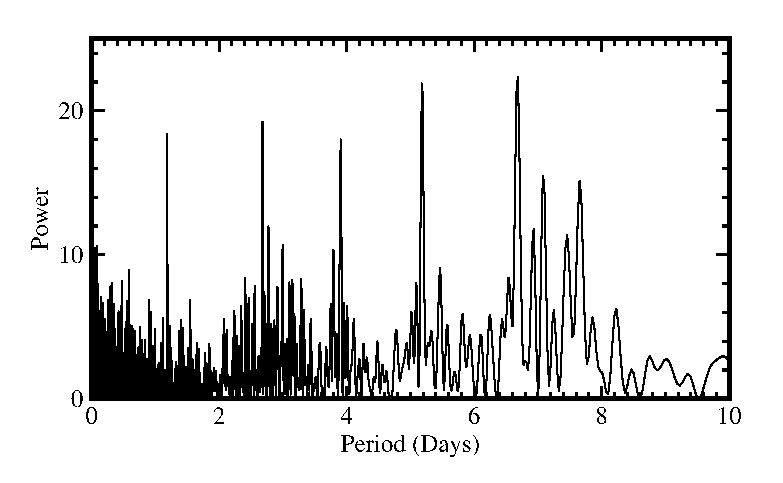
\includegraphics[width=7cm]{LS.eps}
%   \caption{Lomb-Scargle periodogram of the PDC light curve, with the
%     transits masked out. The light curve is rotationally modulated with
%   a period of 1.19 days.}
%   \label{fig:LS}
% \end{figure}

\section{Orbit obliquity from light curve asymmetry}
\label{sec:transit-light-curve}

\subsection{Kepler light curves}
\label{sec:light curve-model}

We make use of all available public Kepler \lcs\ for our analysis of KOI-368. These include 
11 transits (Q0-Q15, more than 1300 day) of Long Cadence (29.4min) data and 2
transits (Q8-Q9) of Short Cadence (58.84s) data .

We start with the raw flux $(\rm SAP\_FLUX)$ obtained from the MAST archive
\footnote{http://archive.stsci.edu/kepler/data$\_$search/search.php}, the out 
of transit variations are corrected by the following steps from 
\citet{Huang:2013}:

a) removal of bad data points;

b) correction of systematics due to various phenomena of the space craft, such as safe modes and tweaks;

c) a set of cosine functions with minimum period of 1 day. 

d) a 7th order polynomial fit on the out of transit parts. 
%\begin{figure}
%  \centering
%  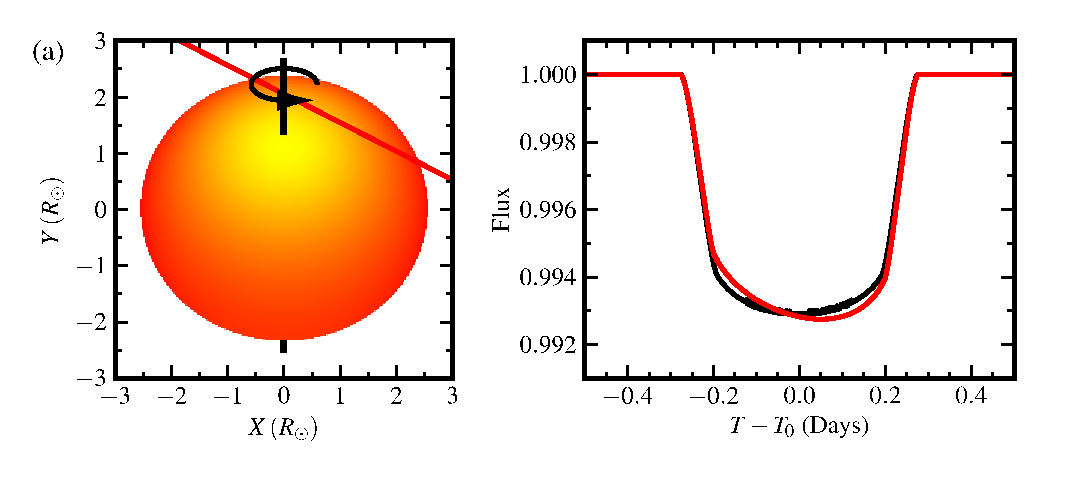
\includegraphics[width=9cm]{obliq_model.eps}
%  \caption{Left panel: flux ratio distribution at the surface of KOI-368 with model 
%  parameters f=0.2, $\beta=1.0$, $i_{\rm rot}=0$. An example planet transit path 
%  with projected obliquity of $45^\circ$ is marked in red. Right panel: the corresponding 
%  light curve is plotted. For comparison, the best fit light curve without 
%    considering gravity darkening is also shown in black. }
%  \label{fig:obliqmodel}
%\end{figure}


\subsection{Gravity darkening modeling}
\label{sec:grav-model}
The gravity darkening model is generated following \citet{Barnes:2009}.
The temperature profile on the stellar surface is determined by the local 
effective gravity $g_{\rm eff}$ \citep{Zeipel:1924}. We use the gravity
darkening coefficient $y$ introduced by \citep{Kopal:1959} which 
directly relates the specific intensity profile of the stellar disk to 
the effective gravity profile: 
%\begin{equation}
%y = \frac{{\rm d}\ln I}{{\rm d}\ln g_{\rm eff}} = \\
%(\frac{\partial\,{\ln I}}{\partial\,{\ln g_{\rm eff}}})_{T_{\rm eff}} \\
%+ (\frac{{\rm d}\ln T_{\rm eff}}{{\rm d}\ln g_{\rm eff}})(\frac{\partial\,{\ln I}}{\partial\,{\ln T_{\rm eff}}})_{g_{\rm eff}}
%\end{equation}.
%Therefore the the ratio of specific intensity $I$ at any position to 
%the intensity at stellar pole $I_{\rm pole}$ can be written as 
\begin{equation}
\frac{I}{I_{\rm pole}} \propto (\frac{g_{\rm eff}}{g_{\rm pole}})^{y}. 
\end{equation}
The effective gravity is defined as 
\begin{equation}
\vec{g}_{\rm eff} = -\Omega_{\rm grav}^2\frac{R_{\rm eq}^3}{R^2}\hat{r} \\ 
+ \Omega_{\rm rot}^2\,R_{\perp}\hat{r_{\perp}}
\end{equation}
We define $\Omega_{\rm rot}$ as the stellar rotation rate in radians 
per second and $\Omega_{\rm grav} = \sqrt(GM/R_{\rm eq}^3)$ to represent the angular velocity due to 
gravity at the equator. 
The definition of the other symbols follow the Eq.10 of \citet{Barnes:2009}, in 
which $G$ is the gravitational constant, $M$ is the mass of the star, $R$ 
and $R_{\perp}$ are the distance from the stellar center and stellar 
rotation axis to the point of question, respectively. $\hat{r}$ and 
$\hat{r_{\perp}}$ are unit vectors indicate the directions of $R$ and 
$R_{\perp}$. 
The effective gravity profile $g_{\rm eff}/g_{\rm pole}$ at the
stellar surface is then only a function of the oblation of the star $f=(R_{\rm eq}-R_{\rm pole})/R_{\rm eq}$, 
the normalized position parameters $r$, $\theta$, and the non-dimension measure of the 
rotation rate ($w=\Omega_{\rm rot}/\Omega_{\rm grav}=v_{\rm rot}^2(R_{\star}/M_{\star})$). 
Since $M_{\star}$ depends proportionally to $R_{\star}$ in spectrum fitting 
of this spectra type region, the uncertainty in the gravity darkening calculation depends weakly on the absolute number of stellar mass and radius. It mainly comes from the stellar oblation $f$ and the rotation velocity 
$v_{\rm rot}$. We use the gravity darkening coefficient computed 
for Kepler band using ATLAS code from \citet{Claret:2011}. By assuming the 
distribution of errors in the stellar parameters to be gaussian, we obtain 
the gravity darkening parameter $y$ to be $0.525$ (later fitted for in Section~\ref{sec:model-fitting}). In Figure~\ref{fig:lightcurve}(a), 
we demonstrate the flux profile computed for KOI-368 system. If the planet crosses the hotter pole to colder 
equator during its transits, the transit \lcs\ will show asymmetry depending 
on the misalignment between the planet orbit and stellar rotation axis.

\begin{figure}
  \centering
  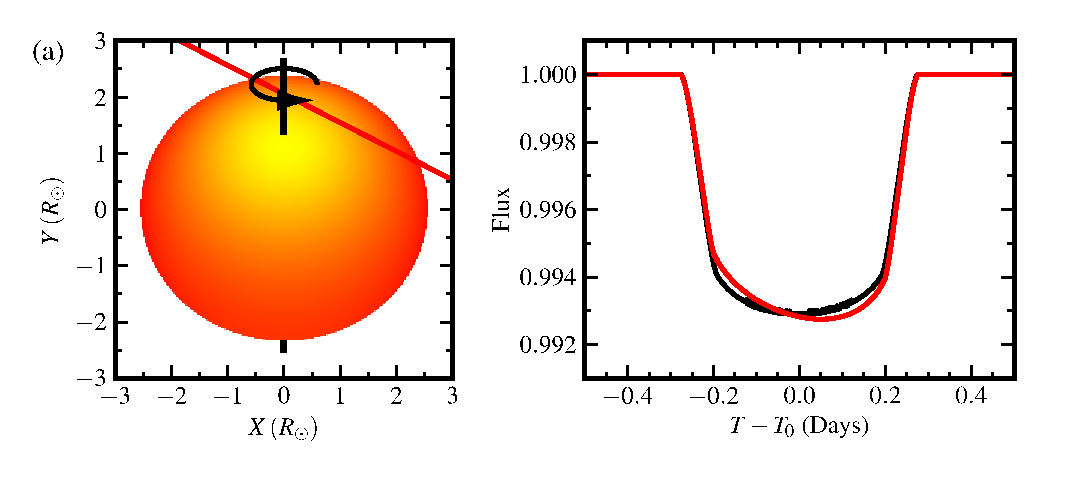
\includegraphics[width=9cm]{obliq_model.eps}
  \includegraphics[width=9cm]{lightcurve.eps}
  \caption{(a) The flux ratio distribution at the surface of KOI-368 is plotted on the left, with 
  $i_\text{rot}=45^\circ$ and exaggerated oblation parameters of $f=0.2$, $y=1.0$. An example planet transit path 
  with projected obliquity of $30^\circ$ is marked in red. The corresponding 
  light curve is plotted on the right (in red). This is the best fit configuration
  for KOI-368.01. For comparison, the best fit light curve without 
    considering gravity darkening is also shown in black. 
  (b) Phase folded transit light curve of KOI-368.01 is plotted. Long
    cadence observations are plotted in black, short cadence in
    green. The best fit standard transit model is
    plotted in blue, gravity darkened model in red. These two models are
    indistinguishable at this scale. (c) Residuals to the
    standard transit model are plotted. The long cadence data are
    plotted in full as gray dots. Long cadence data binned to 1 hour
    intervals are plotted in black, binned short cadence residuals in green. (d)
    Residuals to the gravity darkened transit model are plotted. (e) The maximum light curve 
    distortions due to eccentricity is plotted in black. For comparison, the binned 
    residuals from (c) are also plotted. Distortions due to eccentricity cannot explain 
    the asymmetry of the observed light curve. Note the scale is different to the previous residual plots. }
  \label{fig:lightcurve}
\end{figure}


\subsection{Fitting of system parameters}
\label{sec:model-fitting}

The transit \lcs\ are modeled using the
\citet{Nelson1972} model, implemented in an adaption of the
JKTEBOP code \citep{Proper1981,Southworth2004}. The
relevant free parameters in the transit model are orbital period $P$, transit centre $T_0$,
normalised radius sum $(R_\star+R_p) / a$, radius ratio $R_p/R_\star$,
line of sight inclination $i$. The quadratic limb darkening coefficients,
$c_1$ and $c_2$, are fitted for in an initial minimization routine, with 
starting points from \citet{Sing2010}, then held fixed for 
subsequent analyses. Jump parameters modeling the gravity darkening 
include the sky-projected orbit obliquity angle $\lambda$, stellar oblation factor $f$. The 
projection angle between the stellar rotation axis and line of sight 
$i_\text{rot}$ (with initial value taken from Section~\ref{sec:host-star-parameters}), 
and the gravity darkening exponent $y$ (with initial value taken from Section~\ref{sec:grav-model}). 
A flux offset for each transit event is calculated and removed at each iteration, and is not 
included in the fit parameters. For Kepler long cadence data, the model is 
modified by a 30 minute boxcar smooth. The best fit parameters and the 
posterior probability distribution is explored via a Markov chain Monte Carlo
(MCMC) analysis, using the \emph{emcee} MCMC ensemble sampler
\citep{ForemanMackey2012}. For each transit, we scale the flux errors such
that the reduced $\chi^2$ are at unity. This allows for errors other
than photon noise to be taken into account.

Figure~\ref{fig:lightcurve} plots the phase folded transit light curve of
KOI-368.01 and the best fit standard and gravity darkened models. The best fit
standard model cannot explain the significant in-transit
asymmetry observed. 

The best fit parameters are presented in Table~\ref{tab:params}.
The posterior probability distributions for relevant parameters
are plotted in Figure~\ref{fig:posterior}. We find an inverse dependency
between $\lambda$ and $y$, and a positive dependency between
$\lambda$ and $R_p/R_\star$.

%%% Include parameter table
\begin{deluxetable*}{lrrr}
\tablewidth{0pc}
\tabletypesize{\scriptsize}
\tablecaption{KOI-368 System properties
\label{tab:params}}
\tablehead{
\multicolumn{1}{c}{Parameter} & 
\multicolumn{1}{c}{Spherical Model} &
\multicolumn{1}{c}{Limited Oblate Model} &
\multicolumn{1}{c}{Full Oblate Model} \\
}\startdata
\multicolumn{2}{l}{\textbf{Stellar parameters}}\\ 
$T_\text{eff}$ & $9200\pm500$ & - & -\\
$\log g$ & $4.1\pm0.5$ & - & -\\
$\text{[Fe/H]}$ & $0.0\pm0.5$ & - & -\\
$v \sin i_\text{rot}$ & $100 \pm 10$ & - & -\\
\\
\multicolumn{2}{l}{\textbf{Lightcurve fitting parameters \tablenotemark{1}}} \\ 
Period (Days) & $110.3216229_{-7}^{+3}$& $110.321615_{-6}^{+2}$ & $110.321613_{-7}^{+1}$ \\ 
$T_0$ $(\text{BJD}-2454000)$ & $1030.36382_{-3}^{+2}$& $1030.36407_{-9}^{+6}$ & $1030.36440_{-1}^{+3}$ \\ 
$(R_p+R_\star)/a$ & $0.02101_{-3}^{+1}$& $0.02078_{-5}^{+6}$ & $0.02103_{-2}^{+3}$ \\ 
$Rp/R_\star$ & $0.08401_{-5}^{+4}$ & $0.0866_{-2}^{+1}$ & $0.0854_{-1}^{+1}$ \\
$i$ & $89.209_{-1}^{+2}$ & $89.229_{-4}^{+3}$ & $89.209_{-2}^{+2}$ \\
$f$ & - & $0.064_{-6}^{+3}$ & $0.038_{-2}^{+2}$ \\
$\lambda$ & - & $67_{-7}^{+6}$ & $52_{-7}^{+5}$ \\
$\beta$ & - &- & $0.24_{-3}^{+2}$ \\
$i_\text{rot}$ & - & -  & $25_{-10}^{+4}$ \\
\\
\multicolumn{2}{l}{\textbf{Derived parameters}}\\ 

\enddata
\tablenotetext{1}{Uncertainties quoted are for the last significant figure}
\end{deluxetable*}

\begin{figure*}
  \centering
  \includegraphics[width=12cm]{posterior.eps}
  \caption{Posterior probability distributions showing the correlation
  between the projected obliquity $\lambda$ and stellar oblation $f$,
  radius ratio $R_p/R_\star$, gravity darkening exponent $y$, sky
  projected angle of the stellar rotation axis $i_\text{rot}$. The
  contours mark the 1 and 2$\sigma$ confidence regions. The posterior probability distribution 
for the true obliquity is plotted on the bottom panel.}
  \label{fig:posterior}
\end{figure*}

We find a best fit projected obliquity value of $\lambda = 27_{-13}^{+12\,\circ}$, and the sky 
projected angle of the stellar rotation axis to be $i_\text{rot}=43_{-5}^{+4\, \circ}$. The best fit
true spin-orbit obliquity of KOI-368.01 is $64_{-9} ^{+11\,\circ}$, indicating 
that it is orbiting in a highly inclined orbit. 

Note that due to the degeneracy between the geometries of 
$\lambda$ and $(180^\circ - \lambda)$,  we cannot distinguish between prograde and retrograde
orbits using this method. For the remaining discussion, we arbitarily assume a
prograde orbit. 

We also derive a planet radius of $2.1\pm0.2\,R_\text{Jup}$, larger than the 
Kepler catalogued radius of $1.8\pm 0.8\, R_\text{Jup}$, primarily due to
differences in the adopted host stellar radius values. However, the stellar 
parameters are not well defined, and the uncertainties on the host and planet radii
may be underestimated.

\subsection{Asymmetry from eccentricity}
\label{sec:asymm-from-eccentr}

A highly eccentric orbit can also cause asymmetric distortions to the
transit light curve. An eccentric orbit distorts the light curve by
changing the velocity of the planet through the transit. We explore the
possibility that the light curve distortions observed for KOI-368.01
are due to an eccentric instead of an oblique orbit.

Following \citet{Barnes2007}, we can constrain the change in velocity through a transit
$(\Delta v)$ by measuring the difference
in the duration of ingress and egress $(\Delta t)$,
\begin{equation}
  \Delta v \approx v^2 \frac{\Delta t \cos \left( \sin^{-1} b \right)}{R_p}
\end{equation}
where $b = a \cos i/R_\star = 0.7$ is the transit impact parameter, and $v =
\sqrt{G M_\star / a} = 43.3\,\text{kms}^{-1}$. Using
the short cadence data, we measure ingress and egress durations to be
equal within errors of 0.7 minutes, constraining the maximum
possible change in velocity to be $\Delta v <
0.5\,\text{kms}^{-1}$. Figure~\ref{fig:lightcurve}(e) plots the difference 
between such an eccentric orbit light curve and its best fit circular orbit
light curve. The maximum in-transit distortions are $10
\times$ smaller than that for the oblique orbit model. The maximum
distortions during ingress and egress are $5\times$ smaller than that
for the oblique orbit model, and are not consistent in shape to that
observed for KOI-368.01. The light curve distortions for KOI-368.01
therefore cannot be explained by an eccentric orbit.
%
%\begin{figure}[h!]
%  \centering
%  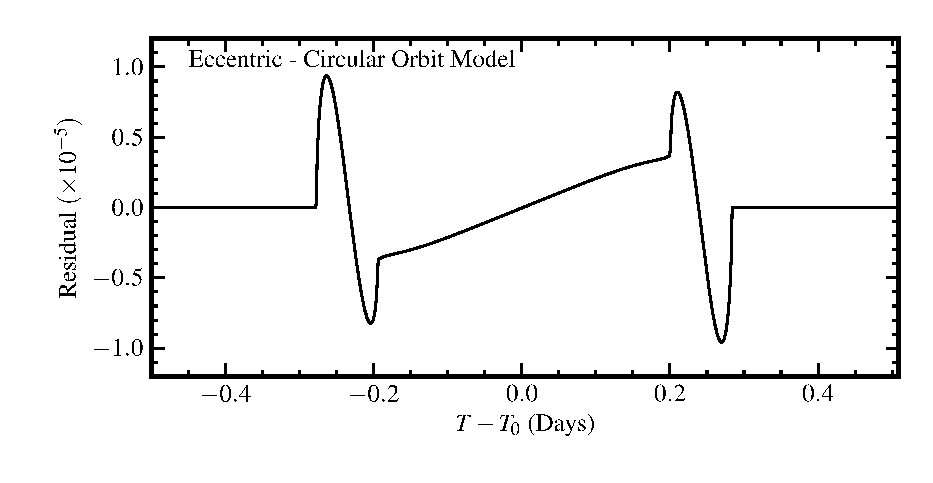
\includegraphics[width=7cm]{ecc_model.eps}
%  \caption{The maximum light curve distortions due to a
%    eccentric orbit for KOI-368.01 are plotted as residuals to its
%    best fit circular orbit model. The maximum velocity change is
%    determined by measuring the difference in the ingress and egress
%    duration. Eccentricity cannot explain the observe light curve
%    asymmetry (Figure~\ref{fig:light curve}, middle panel).}
%  \label{fig:ecc_model}
%\end{figure}

\section{Nature of the KOI-368 system}
\label{sec:system-properties}

\subsection{Excluding blend scenarios}
\label{sec:excluding-blends}

To establish the nature of KOI-368.01, we investigate in the 
false positive scenarios of this system. We use the image from APO 3.5m 
Echelle Slitviewer camera to rule out close-by bright companions. The 
camera has a field of view of 63.6$\arcsec$ and the pixel scale is 0.133\pxs. 
The closest companion brighter than 20 mag is more than 20$\arcsec$ away from KOI-368 (See Figure \ref{fig:APO}). No candidate is found to be 
a possible source of background blend. 

\begin{figure}
\subfigure[]
{
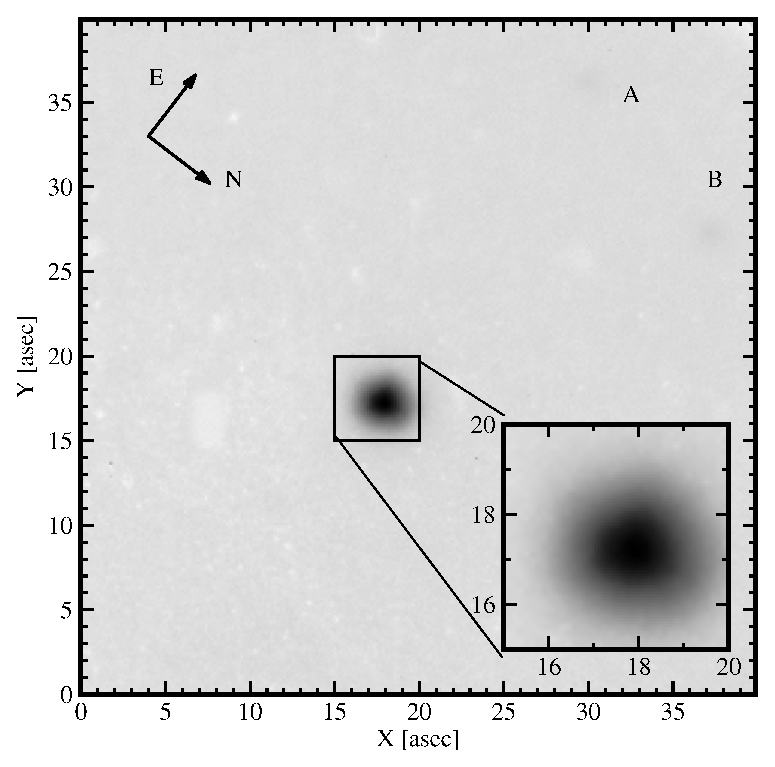
\includegraphics[width=0.4\linewidth]{APOimage_large.eps}
\label{fig:APO}
}
\subfigure[]{
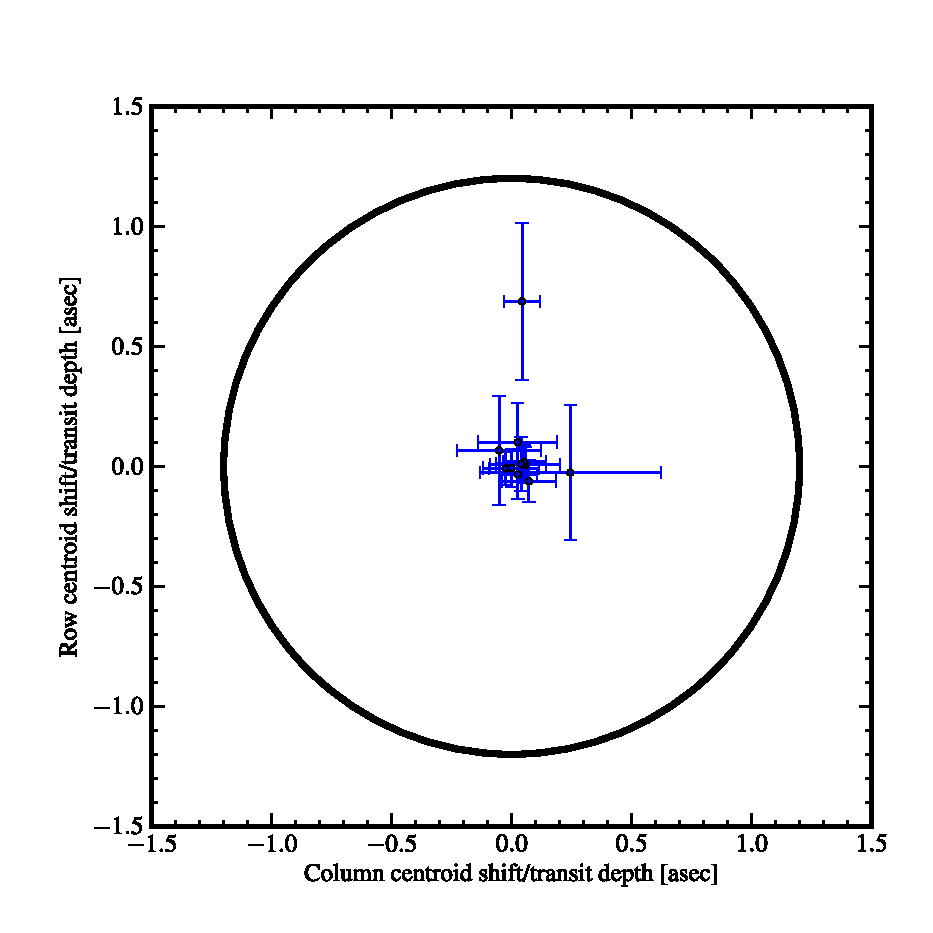
\includegraphics[width=0.45\linewidth]{centroid.eps}
\label{fig:centroid}
}
\caption{
Left Panel: Image of KOI-368 from APO 3.5\,m Echelle Slitviewer 
camera, within $40\times40$\sqarcsec\ area. The two companions  
brighter than 20 magnitude in this region are marked out as A 
and B. Both are around 20$\arcsec$ away. Bottom right shows 
the detail of the target PSF. The half width radius of the 
PSF is 1$\arcsec$. The shape of PSF is not visibily elongated. 
Right Panel: Centroids analysis of KOI-368. We show the 
transit depth normalized centroids displacement between in-transit and 
out-transit for all the 11 transits observed by Kepler Long Cadence data. 
This indicates that the transit signal must be from source within 1$\arcsec$ 
(the black circle). 
\label{fig:FP}
}
\end{figure}

We are able to use the upper limit of centroid displacement to rule out the 
possibility that the transit signal is mimicked by background binaries. We 
use the flux weighted first momentum centroids produced by Kepler 
pipeline. The long time range trend in centroids due to the motion of 
the space craft is corrected by a 7-th order polynomial on each quarter 
of the Long Cadence data. For each Long Cadence transit, we compare the 
centroids of star during the transit with the centroids before and after the
transit (within a window of width the same as the transit duration). The 
displacements between the mean centroids of the in-transit part and the 
out-of-transit part weighted by the transit depth 
\citep{Chaplin:2013} are shown in Figure \ref{fig:centroid}. The error-bars 
are computed with the error propagation rule by assuming the centroids in 
each window follows a Gaussian distribution. The analysis shows that the 
signal could not be from a source farther than 1$\arcsec$ away from the star 
KOI-368.  

\subsection{Searching for secondary eclipses}
\label{sec:nature-companion}

To constrain the temperature of KOI-368.01, we search for secondary eclipses in 
the \emph{Kepler} long cadence light curve. Whilst an eclipse is only guaranteed 
for circular orbits, our discussion in Section~\ref{sec:system-eccentricity} shows that the orbit of KOI-368.01 is
likely of low eccentricity, suggesting a high likelihood of secondary eclipse for the companion.
The light curves are first modified 
by masking out the primary transit and removing large scale variations using a 
cosine filter with minimum width of 1 day. We then perform a grid
search for a secondary eclipse in the phase space between 0.05 and
0.95. No secondary eclipses are detected. We can rule out the presence of any 
secondary eclipse event with depth $>10^{-5}$. We constrain the
temperature of the orbiting companion using MARCS model spectra \citep{Gustafsson:2008} 
to be $< 2700\,\text{K}$, indicating that it must be of substellar nature.

\subsection{Searching for transit-timing variations}
\label{sec:ttv}

For all the 11 transits from Long Cadence data, we fit for their transit 
centers as independent parameters to perform a transit timing analysis. 
All but one of the transit centers from Long Cadence data are consistent with a strictly 
periodic solution within an 1-$\sigma$ error-bar. 
The 9th transit from the epoch has a deviation at 
around 1.2-$\sigma$.
We conclude this system does not have high amplitude Transit Timing Variation. 

%\begin{figure}
%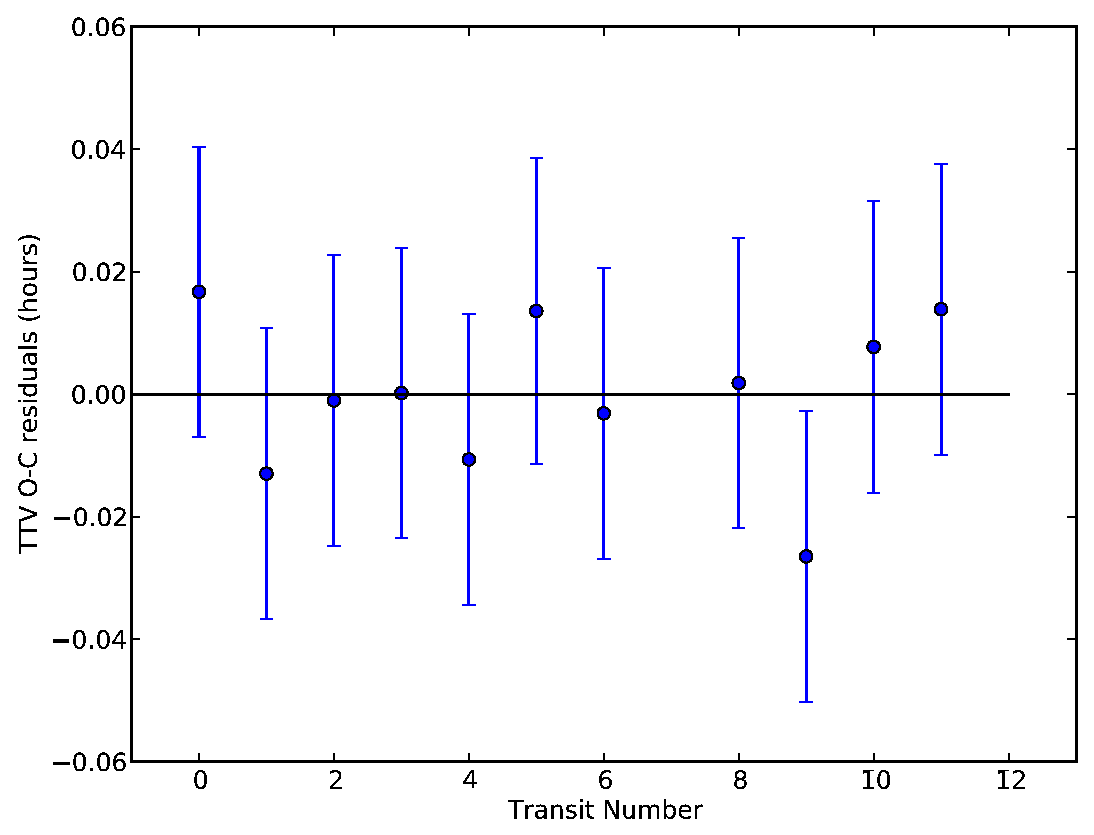
\includegraphics[width=0.9\linewidth]{TTV.eps}
%\caption{ The transit timing analysis of KOI-368.01. All the transit centers 
%(except the 9th transit) from Long Cadence data are consistent with a strictly 
%periodic solution within an 1-$sigma$ error-bar. 
%\label{fig:TTV}}
%\end{figure}

\subsection{Eccentricity of KOI-368.01}
\label{sec:system-eccentricity}

The system eccentricity can be constrained by comparing the measured
transit duration $(t_\text{obs}=13.2\,\text{hours})$ against that expected for a circular
orbit \citep[e.g.][]{Barnes2007,Burke2008,Kane2012}. Adopting host star
parameters of $M_\star = 2.5\pm0.1\,M_\odot$ and $R_\star = 2.5\pm0.2\,R_\odot$
(Section \S\ref{sec:host-star-parameters}), the expected circular orbit 
transit duration is $t_\text{circ} =12.5\,\text{hours}$. Following 
\citet{Burke2008}, we solve for $e$ in
\begin{equation}
  \label{eq:ecc}
  \frac{t_\text{obs}}{t_\text{circ}} = \frac{\sqrt{1-e^2}}{1+e \cos(\omega-\pi/2)}\,,
\end{equation}
and find that $e = 0.07^{+0.18}_{-0.07}$, with errors governed by the uncertainty in the host star radius. Note that we eliminated the degenerate solution to Equation~\ref{eq:ecc} by constraining the eccentricity using Section~\ref{sec:asymm-from-eccentr}. 

\section{Discussion}
\label{sec:discussion}

We measured the asymmetry in the transit light curve of KOI-368.01, and found it to be orbiting in a highly 
inclined plane of $64_{-9} ^{+11\,\circ}$. In the context of existing systems, KOI-368.01 is distinct in 
both host star temperature and period (Figure~\ref{fig:periodobliq}). 

KOI-368 is the hottest host star to date for systems with spin-orbit measurements. It lies well beyond the radiative interior threshold for early-type stars, and the system obeys the empirical bi-modality that radiative stars host high obliquity companions \citep{Winn:2010}. 

With a period of 110.3 days, it is one of the longest period planets for which spin-orbit alignment has been measured. 
Unlike the stable, tightly packed multi-planet systems that 
are star-disk aligned, such as Kepler-25 and 30 \citep{Sanchis-Ojeda:2012,Albrecht:2013}, there is only one other object with obliquity measured outside an orbit of 30 days. Objects in the long period range are subjected to weaker tidal influence from their host stars, therefore their current dynamics is more related to the formation history. HD80606b, the only other long period single planetary system with obliquity measured \citep{Moutou:2009,Winn:2009}, has an almost identical period and projected orbit
obliquity as KOI-368.01, but is highly eccentric $(e=0.93)$. The high eccentricity and obliquity
of the HD80606b can be explained satisfiable with Kozai cycle excited
by its main-sequence companion 1000 AU away \citep{WuMurray:2003, FabryckyTremaine:2007}. 
Curiously, we constrain the eccentricity of the KOI-368 system to be much 
lower, $e = 0.07^{+0.18}_{-0.07}$. If Kozai cycle is also responsible for this high obliquity, the low eccentricity put it in a ``quenched" stage of the migration. Following Equation
12 of \citet{Socrates:2012}, we can rule out solar type 
companion within 100 AU or stellar mass companion within 50 AU.
Considering the age of the system is fairly young ($\sim$250 
Myrs, see Table 1.) and that the typical eccentricity damping timescale 
is 2-3 Gyrs, this system is likely to have formed differently 
to HD80606b. However, we shall remind readers to be cautious with the uncertainties in 
eccentricity, which mainly comes from the large uncertainties in the stellar 
radius, and may be underestimated. Accurate stellar parameters from asteroseismology, 
or a future parallax measurement from \emph{GAIA}, will settle this uncertainty.   

%%%Population
 %Its orbit and obliquity is comparable to HD 80606b 
%\citep{Moutou:2009,Winn:2009}, the only other long period %single-planet system exhibiting 
%spin-orbit misalignment, although the low eccentricity of KOI%-368.01 may point towards a different 
%migration mechanism. Unlike the stable, tightly packed multi%-planet systems that are star-disk aligned, 
%such as Kepler-25 and 30 \citep{Sanchis-Ojeda:2012,Albrecht:2013}, objects like KOI-368.01 and HD 80606b 
%may be the first examples of systems observed in the process of migration. In terms of host star 
%temperature, 
%[Is this important for long period planets?] 

\begin{figure}
  \centering
  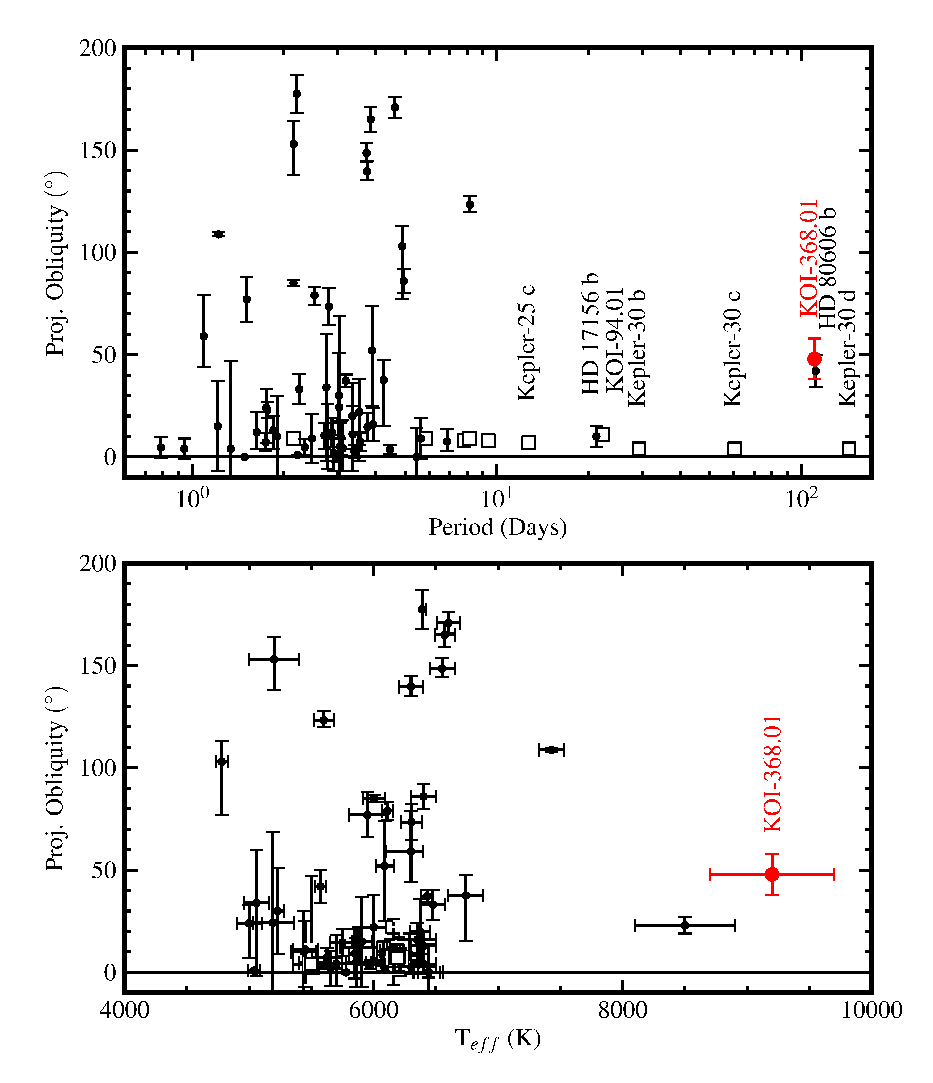
\includegraphics[width=9cm]{period_obliq.eps}
  \caption{The obliquities of planetary systems\footnote{From \url{http://exoplanets.org/}} are plotted against their orbital period (Top) and host star effective temperature (Bottom). Planets with periods longer than 10 days are labelled in the top panel. Planets in single planet systems are marked by solid points, in multi-planet systems marked by open squares. For KOI-368.01, we plot its true obliquity in red.}
  \label{fig:periodobliq}
\end{figure}

It is also important to highlight the advantages of this technique in measuring spin-orbit alignments 
for long-period planets. Whilst the obliquity of HD 80606b was measured using ground-based RM observations, 
the long transit duration and careful planning required stretches the technique to its limits. 
Measuring spin-orbit alignment via star-spot crossings, the only other technique to yield results for 
such long-period planets to date, is severely biased towards planets in perfect spin-orbit alignment, 
and will not identify systems like KOI-368. The high-precision photometry from \emph{Kepler} means that 
the measurement of orbit obliquity from planets about rapidly rotating stars, in conjunction with the 
measurement of the sky-projected angle of the stellar rotation axis, are crucial in exploring the dynamics 
of long-period systems.

\bibliographystyle{apj}
\bibliography{mybibfile}

\end{document}
